\chapter{Analyzing Comorbidity of Developmental Disorders }
The actual data is divided into two types, the first deals with children who are diagnosed with ASD and both ASD and ADHD and the second deals with children who are diagnosed with VCFS, ASD and both these disorders. In the first half go this chapter using the first data, the comorbid disorders ASD and ADHD are analyzed and then in the second half of this chapter comorbid disorders VCFS and ASD are analyzed. Different supervised and unsupervised machine learning techniques will be applied in both the sections to build models and results obtained will be analyzed. Also, analysis will be done on the features selected in chapter 3 by building models using these features and comparing them with other models. 
\section{ASD and ADHD Comorbidity}
The data being used to analyze ASD and ADHD comorbidity consists of 254 subjects who have been diagnosed with ASD, out of which 63 subjects have ADHD as well. This data consists of 190 males and 64 females where 53 males and 10 females have ADHD along with ASD. Initially, $K$-Means algorithm with PCA has been applied to check if these two groups could be distinguished by our $K$-means algorithm. However, our means algorithm was not able to distinguish these two groups of children in both two and three dimensions. There was an overlap in the feature values and our unsupervised learning technique couldn’t result in pure clusters even as we increased the size of $k$ to 9. So, supervised learning techniques were applied on the data and this is discussed in the next sub section.

\subsection{Supervised Learning Techniques to predict ADHD in Autistic children}
The data used for this analysis has already been preprocessed in the chapter 3, now this data is loaded into WEKA and different machine learning classifiers in WEKA are used to build our models. The different Machine Learning classifiers used for our analysis are Naive Bayes, Logistic Regression, Random Forest, Support Vector Machines and K-Nearest Neighbors. These algorithms have been applied to our data to build models as they are suitable for data and these algorithms work well with the type of data that we have. The results obtained from our machine learning algorithms on our data is given below in table \ref{table:51}.
\begin{table}[h]
\begin{center}
\begin{tabular}{|l|c|c|c|c|}
\hline
\textbf{ML Algorithm} & \textbf{Accuracy}&	\textbf{Precision}&	\textbf{Recall}&	\textbf{ROC Area}\\
\hline \hline
Naive Bayes	&92.126\%&	0.922&	0.921&	0.956\\
\hline
Logistic Regression&	83.46\%&	0.838&	0.835&	0.864\\
\hline
Random Forest&	96.063\%&	0.960&	0.961&	0.965\\
\hline
Support Vector Machine&	92.9134\%&	0.929&	0.929&	0.900\\
\hline
$K$ Nearest Neighbors ($n$=3)&	90.1575\%&	0.913&	0.902&	0.937\\
\hline
\end{tabular}
\end{center}
\caption{Results of Supervised Learning Techniques to predict ADHD in Autistic children}
\label{table:51}
\end{table}

From the results obtained by different machine learning algorithms it can be seen that Random forest is performing well. The Random Forest algorithm is able to classify 244 subjects correctly. For more information on how our model is performing, we analyzed how Random Forest algorithm performs with both the groups and the model had a precision of 97\% and recall of 98\% for children with ASD only and precision of 93.4\% and 90\% for children with ASD and ADHD. It could be seen that the model is performing well with both the groups. So, Random Forest algorithm yields the best results for our model and could be considered to be the best model. For further analysis of features, the features can successfully distinguish our two groups, the features selected in chapter 3 are used to build are models and then the results by LASSO, ReliefF  and RFE feature selection algorithms are shown in table \ref{table:52},\ref{table:53} and \ref{table:54} respectively.
\begin{table}[h]
\begin{center}
\begin{tabular}{|l|c|c|c|c|}
\hline
\textbf{ML Algorithm} & \textbf{Accuracy(\%)}&	\textbf{Precision(\%)}&	\textbf{Recall(\%)}&	\textbf{ROC Area}\\
\hline \hline
Naive Bayes	&91.73&	91.7&	91.7&	0.930\\
\hline
Logistic Regression&	91.7&	91.6&	91.7&	0.959\\
\hline
Random Forest&	95.669&	95.7&	95.7&	0.978\\
\hline
Support Vector Machine&	92.126&	92.5&	92.1&	0.910\\
\hline
$K$ Nearest Neighbors($n$=3)&	93.3071&	93.6&	93.3&	0.946\\
\hline
\end{tabular}
\end{center}
\caption{Results of Supervised Learning Techniques to predict ADHD in Autistic children by LASSO}
\label{table:52}
\end{table}

Random Forest is performing well for diagnosing the comorbidity and K-nearest Neighbor(n=3) is also doing a good job. So, the features selected by LASSO could be used to distinguish if an autistic child has ADHD or not. On the other hand, the features selected by the ReliefF are not doing a good job at analyzing the comorbidity. The best model is Support Vector Machines with a low accuracy of 75\%.
\begin{table}[h]
\begin{center}
\begin{tabular}{|l|c|c|c|c|}
\hline
\textbf{ML Algorithm} & \textbf{Accuracy(\%)}&	\textbf{Precision(\%)}&	\textbf{Recall(\%)}&	\textbf{ROC Area}\\
\hline \hline
Naive Bayes	&64.17&	76.1&	64.2&	0.721\\
\hline
Logistic Regression&	72.83&	71.3&	72.3&	0.705\\
\hline
Random Forest&	72.83&	71.3&	72.3&	0.705\\
\hline
Support Vector Machine&	75.19&	56.5&	75.2&	0.5\\
\hline
$K$ Nearest Neighbors($n$=3)&	74.409&	72.5&	74.4	&0.662\\
\hline
\end{tabular}
\end{center}
\caption{Results of Supervised Learning Techniques to predict ADHD in Autistic children by ReliefF}
\label{table:53}
\end{table}

The features selected by RFE are able to distinguish the two subgroups of children extremely well. From table \ref{table:54}, it can be seen that all the models are consistent when diagnosing the children. Hence, the ADI parent-oriented features are the best features to diagnose these two subgroups of children.
\begin{table}[h]
\begin{center}
\begin{tabular}{|l|c|c|c|c|}
\hline
\textbf{ML Algorithm} & \textbf{Accuracy(\%)}&	\textbf{Precision(\%)}&	\textbf{Recall(\%)}&	\textbf{ROC Area}\\
\hline \hline
Naive Bayes	&694.488	&94.6	&94.5	&0.937\\
\hline
Logistic Regression&94.4 &	94.6&	94.5&	0.953\\
\hline
Random Forest&94.488 &	94.6 &	94.5 &	0.942\\
\hline
Support Vector Machine&	94.488 &	94.6	&94.5 &	0.931\\
\hline
$K$ Nearest Neighbors($n$=3)&92.9134 &	93.2 &	92.9 &	0.929\\
\hline
\end{tabular}
\end{center}
\caption{Results of Supervised Learning Techniques to predict ADHD in Autistic children by RFE}
\label{table:54}
\end{table}

J48 algorithm is used to best summarize our model using the ADI features and the pruned tree in shown in figure \ref{fig:51} has an accuracy of 94.4\% and precision and recall range from 88\% to 96\%. The J48 results in figure \ref{fig:52} are obtained using the BASC and the VINE parent-oriented review. Th accuracy of the resulting model is 80\%. When comparing both these trees, it can be seen that the J48 pruned tree resulting from ADI parent-oriented reviews is better than the one from BASC and VINE. Therefore, ADI parent-oriented review is better than BASC or VINE parent-oriented review at distinguishing if an autistic child has ADHD or not.
\begin{figure}
\centering
  {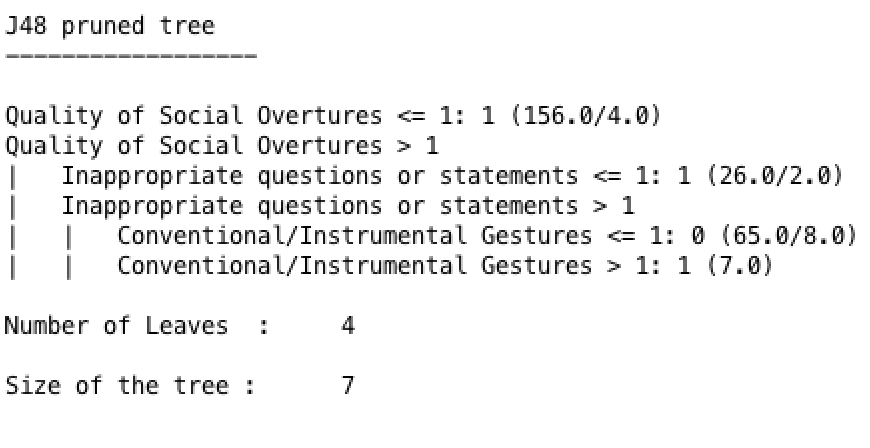
\includegraphics[width=0.6\textwidth]{Figures/Figure_5_1.png}}
  \caption{J48 pruned tree with ADI parent-oriented review}
  \label{fig:51}
\end{figure}

\begin{figure}
\centering
  {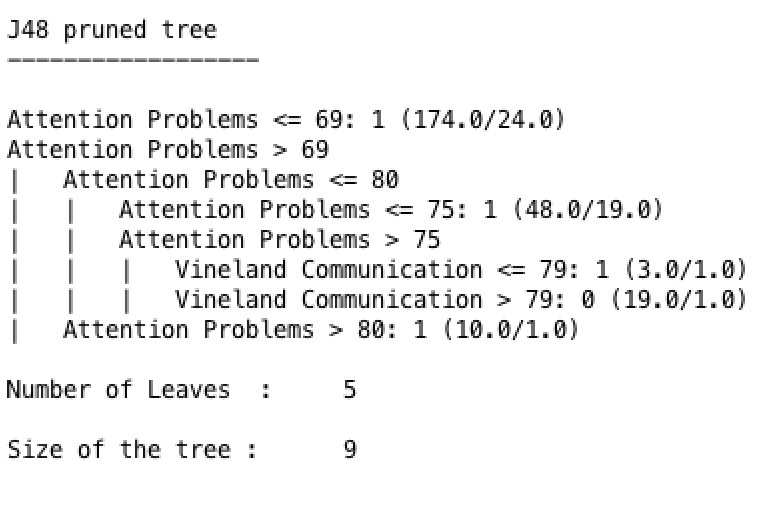
\includegraphics[width=0.6\textwidth]{Figures/Figure_5_2.png}}
  \caption{J48 pruned tree with BASC and VINE parent-oriented review}
  \label{fig:52}
\end{figure}

\subsection{Individual Feature Sets Analysis}
As the date consists of four different types of features, Random Forest model is trained on each of these feature sets. The four different feature sets are IQ, ADI BASC and VINE feature set. The results of these Random Forest models are obtained in table \ref{table:55}. When analyzing the IQ feature set, additional data from the ABIDE and ADHD-200 dataset was taken. The subjects from these datasets were taken by random sampling strategy. So, when the Random Forest model was trained on these there groups of data(ASD, ADHD, ASD+ADHD), the performance of the model dropped. It had an accuracy of 60\% which is lesser compared to the IQ feature set analysis of groups(ASD, ASD+ADHD). Therefore, from the models obtained, IQ of the child is not a clear indicator of the diagnosis of the child, that is the ASD and ADHD comorbidity cannot be analyzed with IQ.

\begin{table}[h]
\begin{center}
\begin{tabular}{|l|c|c|c|c|}
\hline
\textbf{Feature Set} & \textbf{Accuracy(\%)}&	\textbf{Precision(\%)}&	\textbf{Recall(\%)}&	\textbf{ROC Area}\\
\hline \hline
IQ	&65.7\%	 &0.628 &	0.657&	0.588\\
\hline
ADI& 96\% &	0.960 &	0.961 &	0.966\\
\hline
BASC &75.98\%	&0.726	&0.760	&0.727\\
\hline
VINE&	73.6\%	&0.562 &	0.736 &	0.557\\
\hline
\end{tabular}
\end{center}
\caption{Random Forest algorithm with different feature sets.}
\label{table:55}
\end{table}

By analyzing the models, it can be seen that ADI parent-oriented review is performing better than the other three feature sets. Similar results were obtained when analyzing the feature selection models. Therefore, for distinguishing the two groups ADI parent-oriented review plays a vital and only this review could be used to diagnose the children as well.

\subsection{Ensemble methods to predict ADHD in Autistic children}
Ada Boosting and Logit Boosting are two different types of boosting techniques that have been used on our data. Ada Boost uses weights to give more importance to certain variables over others. It is an iterative method that classifies data in the best way possible at each step. Logit Boosting also works similar to Ada Boost however, the cost function through which weights are given to variables varies in both these algorithms. For logit boosting the cost function is of that applied to logistic regression and minimizes the logistic loss in (1) and the training error function minimized by Ada boosting algorithm at each iteration t is given in (2).
$$
\sum_{i} \log (1+e^{-y_{i}f(x_{i})})\eqno{(1)}
$$

$$
\sum_{i} E[F_{t-1}(x_{i})+ \alpha_{t}h(x_{i})] \eqno{(2)}
$$
The Ada Boosting technique took 5 iterations and the accuracy of the model is 90.5\% while the ROC Area is 0.951. Also, the precision and recall for ASD+ADHD group is 76\% and 92\% and for the ASD group is 97\% and 90\%. The features selected by the Ada Boosting algorithm at each iteration are given below:
\begin{compactenum}
\item Quality of social overtures- According to Ada Boosting if the value of this feature is equal to 2, then with 60\% confidence the class is ASD+ADHD. However, when the feature value is not equal to 2, then with 97\% confidence it is ASD. This was selected in the first iteration with weight of 1.59.
\item Attention Problems- When the subjects feature value is greater than 69.5 than it belongs to ASD class with 52\% confidence, but it has higher confidence of 92\% when it is less than or equal to 69.5. This was selected in iteration 2 and 4 with weights of 1.47 and 1.24 respectively.
\item Offering to share- When the subjects feature value is not equal to 1 than it belongs to class ASD+ADHD with 63\% confidence. On the other hand, when feature value is equal to 1, then it belongs to ASD class with 97\% accuracy. This was selected in iteration 3 with weight of 0.9.
\item Inappropriate questions or statements- When the subjects feature value is not equal to 2 than it belongs to class ASD with 87\% confidence. However, when feature value is equal to 2, then it belongs to ASD+ADHD class with 66\% accuracy. This was selected in iteration 3 5 with weight of 1.18.
\end{compactenum}

Similarly, when Logit Boosting technique has been applied to the data, the accuracy of the model is 92\% and the ROC Area is 0.949. The precision and recall for the ASD class is 94\% each. On the other hand, the precision and recall for the ASD+ADHD class is 84\% each. The features selected by Boosting technique at each iteration is given below:
\begin{compactenum}
\item Quality of social overtures
\item Inappropriate questions or statements
\item Attention Problems
\item Response to Approaches of other children
\item Conventional/Instrumental Gestures
\end{compactenum}

\subsection{Observations}
During the comparison of all the three feature selection algorithms, it can be seen that the variable “Vineland Socialization” of the VINE is most important over others as two of our feature selection algorithms have selected it. Similarly, “Attention Problems” variable from BASC and “Quality of social overtures” and “Inappropriate questions or statements” variables from ADI. These variables that our algorithm has selected are actually the most important signs of ASD and ADHD in individuals when compared to other signs.

The results obtained after applying boosting techniques show that rules can be made for these features in the form of decision stumps, which will help in better diagnosis. Also, Logit Boosting performed better with our data over Ada Boosting. The most important features that have been selected by majority of our machine learning algorithms are given below:
\begin{compactenum}
\item Quality of social overtures
\item Inappropriate questions or statements
\item Attention Problems
\item Conventional/Instrumental Gestures
\end{compactenum}

Our data doesn’t contain control groups, so the false diagnosis of these disorders was not a problem. But, even in the existing data false negatives of ADHD are minimal, this shows that machine learning is doing a good job at predicting if autistic children are showing signs of ADHD or not. It shows positive signs of being able to distinguish ASD patients from the ASD+ADHD patients with limited variables. These techniques could be applied to larger datasets and our models would be more generalized. Hence, even though these methods are not ready to be used in real-time, the results of our study indicate that in the near future, machine learning will show promising results in the clinical diagnosis of developmental disorders specifically those that do not have genetic relations like ASD and ADHD.

\section{VCFS and ASD Comorbidity}
When analyzing the comorbid disorders ASD and VCFS, the data has been separated for this purpose. It consists of subjects who are diagnosed with ASD, VCFS and both these disorders together. On this modifies data, different machine learning algorithms have been applied. Also, the features selected by different feature selection algorithms in chapter 3 are also used to build models. The observations made in this analysis are discussed in the next section.
\subsection{Applying Supervised Learning Techniques}

The data which consists of the three different class labels that is used for this analysis has already been preprocessed in the chapter 3, now this data is loaded into WEKA and different machine learning classifiers in WEKA are used to build our models. These algorithms have been applied to our data to build models as they are suitable for data and these algorithms work well with the type of data that we have. The results obtained from our machine learning algorithms on our data is given below in table \ref{table:56}. \nomenclature{SVM}{Support Vector Machine}
\begin{table}[h]
\begin{center}
\begin{tabular}{|l|c|c|c|c|}
\hline
\textbf{ML Algorithm} & \textbf{Accuracy(\%)}&	\textbf{Precision(\%)}&	\textbf{Recall(\%)}&	\textbf{ROC Area}\\
\hline \hline
Naive Bayes	&94.11&	0.953&	0.941&	0.994\\
\hline
Logistic Regression&	89.8	&0.902&	0.899&	0.963\\
\hline
Random Forest&96.7 &	0.968 &	0.967	&0.997\\
\hline
Support Vector Machine&97.0	&0.970&	0.971&	0.976\\
\hline
$K$ Nearest Neighbors ($n$=3)&93.7&	0.940&	0.938&	0.980\\
\hline
\end{tabular}
\end{center}
\caption{Supervised Learning techniques for ASD and VCFS comorbidity}
\label{table:56}
\end{table}

By comparing the different supervised learning techniques both SVM and Random Forest algorithms have similar model performance. Also, both these models are better than other machine learning techniques that have been used. When the models are compared based on each of the class labels, then SVMs are better than Random Forest. Using the entire features available for the data, the J48 algorithm summarized our model. The results obtained from our J48 algorithm are shown in figure \ref{figure:53} For further analysis of these comorbid disorders, SVM models are built on each of the features selected by the feature selection algorithms in chapter 3. The results obtained by these SVM models are shown in table \ref{table:57}.
\begin{figure}
\centering
  {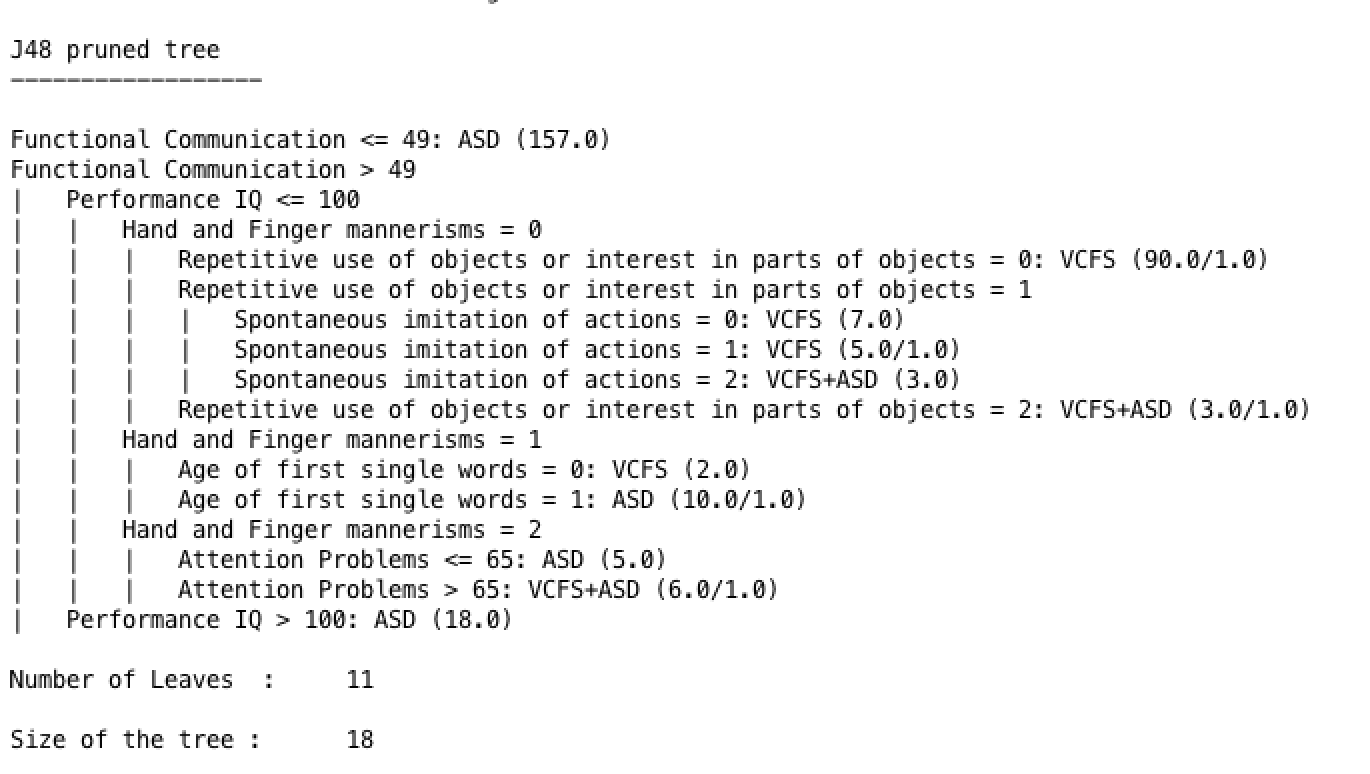
\includegraphics[width=0.6\textwidth]{Figures/Figure_5_3.png}}
  \caption{J48 pruned tree with ADI feature set}
  \label{fig:53}
\end{figure}
\begin{table}[h]
\begin{center}
\begin{tabular}{|l|c|c|c|c|}
\hline
\textbf{Feature Selection Algorithm}& \textbf{Accuracy(\%)}&	\textbf{Precision(\%)}&	\textbf{Recall(\%)}&	\textbf{ROC Area}\\
\hline \hline
LASSO&	62.09&	0.389&	0.621&	0.498\\
\hline
ReliefF&	78.43&	0.765&	0.784&	0.805\\
\hline
RFE&	90.5&	0.873&	0.905&	0.909\\
\hline
\end{tabular}
\end{center}
\caption{Feature Selection Algorithms for ASD and VCFS comorbidity}
\label{table:57}
\end{table}

SVM model trained by RFE features is the best and the performance of the other to models is not comparable to our previous models. If this model was compared to SVM model with entire dataset, it could be seen that the performance of the model has dropped by 7\%.

\subsection{Individual Feature Sets Analysis}
In this section, ASD and VCFS comorbidity is analyzed with respect to each of the individual feature sets present in our data. The SVM model which is performing well with our data is trained on each of the individual feature sets. The results of these models are shown in table \ref{table:58}. By comparing these models, ADI parent oriented reviews model performance is better than other feature sets. However, when compared to the previous models of SVM, the performance is less, but this model could be a better generalization of our data. 
\begin{table}[h]
\begin{center}
\begin{tabular}{|l|c|c|c|c|}
\hline
\textbf{Feature Set}& \textbf{Accuracy(\%)}&	\textbf{Precision(\%)}&	\textbf{Recall(\%)}&	\textbf{ROC Area}\\
\hline \hline
IQ	&63.07\%&	0.566&	0.631&	0.518\\
\hline
ADI& 93.13\%&	0.927&	0.931	&0.936\\
\hline
BASC &84.96\%&	0.841&	0.850&	0.874\\
\hline
VINE&	80.3\%&	0.785&	0.804&	0.825\\
\hline
\end{tabular}
\end{center}
\caption{Random Forest algorithm with different feature sets.}
\label{table:58}
\end{table}

\subsection{Applying Ensemble Methods}
Ada Boosting and Logit Boosting techniques were applied to the ASD and VCFS data and the performance of these models has been analyzed. The accuracy of Ada Boosting technique is 92.15\% and ROC Area is 0.978. The Ada model takes 5 iterations and the features selected at each iteration are given below:
\begin{compactenum}
\item Criteria for Repetitive behaviors and stereotyped patterns- When this feature value is equal to ‘Yes’, then child belongs to the class label ASD with 90\% confidence. However, when the feature value is not ‘Yes’, then child belong to class label VCFS  with 88\% confidence. The weight given to this feature is 2.18.
\item Functional Communication- The subject belongs to the class ASD, when the feature value is less than or equal to 49.5 with 100\% confidence. On the other hand, individuals belongs to class VCFS with less confidence of 54\%, if the feature value is greater than 49.5. The weight assigned to this feature is 1.08.
\item Adaptive Daily Living- The weight for this feature is 0.67. When this feature takes a value less than of equal to 49 subjects belongs to ASD class with 100\% confidence. However, when the value is greater than 49, with 50\% confidence the subjects belongs to the VCFS and ASD class.
\item Vineland Composite- The weight assigned for this feature is 0.4. The class label is VCFS with 42\% confidence, if the feature value is less than 98.5. Also, the class label is ASD with 97\% confidence, if feature value is greater than 98.5
\item Criteria for Communication- When this feature value is equal to ‘Yes’, then subject belongs to the class label VCFS+ASD with 50\% confidence. However, when the feature value is not ‘Yes’, then child belong to class label VCFS  with 64\% confidence. The weight given to this feature is 0.22.
\end{compactenum}
Logit Boosting has a model accuracy of 95.7\% and ROC Area value of .988. It is performing better than Ada boosting. Also, for subjects that both these disorders, the model performance is better. The features selected by Login Boosting are given below:
\begin{compactenum}
\item Functional Communication
\item Criteria for Repetitive behaviors and stereotyped patterns
\item Vineland Daily Living
\item Criteria for Qualitative impairments in reciprocal social interaction
\item Quality of social overtures
\item Adaptive Daily Living
\item Hyperactivity
\item Performance IQ
\item Criteria for Communication
\item Spontaneous imitation of actions
\item Attention Problems
\item Verbal IQ
\item Somatization
\end{compactenum}

\subsection{Observations}
As our data consists of less number of children who are diagnosed with VCFS and ASD, the models that are being trained on this data are able to precisely detect those children. However, it cannot be guaranteed that our models are able to generalize this class label.Our models are doing a good job with the individual diagnosis of ASD and VCFS especially the Support Vector Machine algorithm. The best features which help in analyzing our comorbid disorders are given below:
\begin{compactenum}
\item Functional Communication
\item Criteria for Communication
\item Spontaneous imitation of actions
\item Adaptive Daily Living
\item Criteria for Repetitive behaviors and stereotyped patterns
\item Repetitive use of objects or interest in parts of objects
\end{compactenum}

On comparison of the feature sets, ADI parent-oriented review is better than the other two parent-oriented reviews. Also, the IQ feature set is not good at analyzing the comorbidity of ASD and VCFS. Overall, due to the difference in the class proportions, the machine learning algorithms are not able to categorize when generally. Also, RFE has selected features from ADI parent-oriented reviews and it is better than other feature selection algorithms. When comparing the boosting techniques, Logit is doing better, but it has chosen a variety of features. Therefore, for analyzing ASD and VCFS comorbidity, ADI parent-oriented review provide better generalization and so does the J48 model.